\section{Design viewpoints}

\subsection{Introduction}
    This chapter describes the design viewpoints relevant to this project in detail. Each section will address design concerns related to the design views denoted in section 4.4. Seven design viewpoints will be described:
    \begin{itemize}
        \item Context viewpoint
        \item Composition viewpoint
        \item Dependency viewpoint
        \item Interface viewpoint
        \item Interaction viewpoint
        %\item Algorithm viewpoint
        \item Resource viewpoint
    \end{itemize}

\subsection{Context Viewpoint}
    
    % \subsubsection{Concerns}
    %     As stated in section \ref{desc:context}, the primary concern is that the experience of actors should not inhibit their ability to use the product.
    %     The product targets one user, so each use case will only have one actor.
        
    \subsubsection{Elements}
        \paragraph{Switch subsystem}
           The user shall be able to switch between looping subsystem and modulation subsystem.
          
                \begin{figure}[!ht]
                    \centering
                    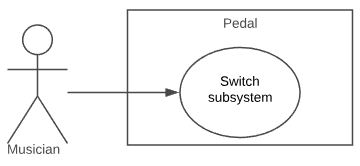
\includegraphics[width=.5\textwidth]{diagrams/use_cases/uc-switch.JPG}
                    \caption{Switch subsystem use case}
                    \label{fig:uc-switch}
                \end{figure}
        \clearpage
        \begin{table}[!ht]
            \centering
            \begin{tabular}{ l l  }
                Use Case & Switch subsystem  \\
                \hline \\
                Use Case Number & 1 \\ \\
                Summary & Musician can switch between the looping subsystem and the modulation subsystem. \\ \\
                Actor & Musician \\ \\
                Trigger & Hardware input: button or switch \\ \\
                
                Pre-Conditions & The pedal must be in either the looping subsystem or the modulation subsystem  \\ \\
                Post-Conditions & If the pedal was initially in the modulation system, it must be in the looping system. \\ 
                & If the pedal was initially in the looping system, it must be in the modulation system. \\ \\
                Assumptions & The pedal is powered on \\ \\
            \end{tabular}
            % \\
            % \caption{Use case: Switch subsystem}
            % \label{tab:uc-switch}
        \end{table}

        \paragraph{Start recording audio} 
        The user shall be able to record audio to playback later.
                    \begin{figure}[!ht]
                \centering
                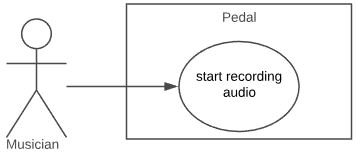
\includegraphics[width=.5\textwidth]{diagrams/use_cases/uc-record-start.JPG}
                \caption{Start recording audio use case}
                \label{fig:uc-record-start }
            \end{figure}
        \begin{table}[!ht]
            \centering
            \begin{tabular}{ l  l  }
                Use Case & Start recording audio  \\ \hline \\
                Use Case Number & 2 \\ \\
                Summary & Musician can start recording audio. \\ \\
                Actor & Musician \\ \\
                Trigger & Hardware input: pedal toggle \\ \\
                Pre-Conditions & The pedal must be in the looping subsystem. \\
                & The looping subsystem must not already be recording. \\ \\
                Post-Conditions & The looping subsystem will be recording incoming audio. \\ \\
                Assumptions & The user has audio input plugged in.\\
            \end{tabular}
            % \\
            % \caption{Use case: Start recording audio}
            % \label{tab:uc-record-start}
        \end{table}
        
        \clearpage
        \paragraph{Stop recording audio} 
            The user shall be able to record audio to playback later.
            \begin{figure}[!ht]
                \centering
                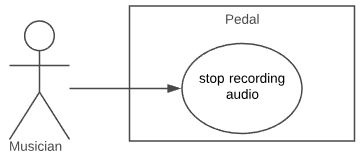
\includegraphics[width=.5\textwidth]{diagrams/use_cases/uc-record-stop.JPG}
                \caption{Stop recording audio use case}
                \label{fig:uc-record-stop }
            \end{figure}
            
            \begin{table}[!ht]
                \centering
                \begin{tabular}{ l  l }
                    Use Case & Stop recording audio  \\
                    \hline \\
                    Use Case Number & 3 \\ \\
                    Summary & Musician can stop recording audio. \\ \\
                    Actor & Musician \\ \\
                    Trigger & Hardware input: pedal toggle \\ \\
                    Pre-Conditions & The pedal must be in the looping subsystem. \\
                    & The looping subsystem must be recording audio. \\ \\
                    Post-Conditions & The looping subsystem will cache the recorded audio. \\ \\
                    Assumptions & The user has audio input plugged in.\\ 
                \end{tabular}
                % \\
                % \caption{Use case: Stop recording audio}
                % \label{tab:uc-record-stop}
            \end{table}
 
      
        \paragraph{Start audio playback} 
            The user shall be able to playback recorded audio.
            \begin{figure}[!ht]
                \centering
                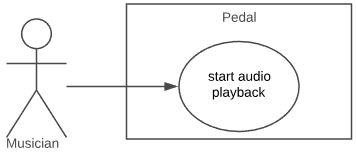
\includegraphics[width=.5\textwidth]{diagrams/use_cases/uc-play-start.JPG}
                \caption{Start audio playback use case}
                \label{fig:uc-play-start}
            \end{figure}
            \clearpage
            \begin{table}[!ht]
                \centering
                \begin{tabular}{l l}
                    Use Case & Start audio playback \\ 
                    \hline \\
                    Use Case Number & 4 \\ \\
                    Summary & Musician can start playing back audio. \\ \\
                    Actor & Musician \\ \\
                    Trigger & Hardware input: pedal toggle \\ \\
                    Pre-Conditions & The pedal must be in the looping subsystem. \\
                    & The looping subsystem must have audio cached. \\ \\
                    Post-Conditions & The looping subsystem will begin audio playback. \\ \\
                    Assumptions & None.\\ 
                \end{tabular}
                % \\
                % \caption{Use case: Start audio playback}
                % \label{tab:uc-play-start}
            \end{table}
            
            \paragraph{Stop audio playback} 
            The user shall be able to stop the playback recorded audio.
            \begin{figure}[!ht]
                \centering
                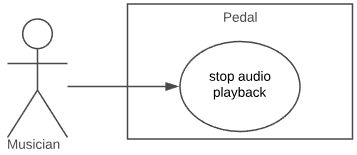
\includegraphics[width=.5\textwidth]{diagrams/use_cases/uc-play-stop.JPG}
                \caption{Stop audio playback use case}
                \label{fig:uc-play-stop}
            \end{figure}
            \begin{table}[!ht]
                \centering
                \begin{tabular}{l l}
                    Use Case & Stop audio playback \\ 
                    \hline \\ 
                    Use Case Number & 5 \\ \\
                    Summary & Musician can stop audio playback. \\ \\
                    Actor & Musician \\ \\
                    Trigger & Hardware input: pedal toggle \\ \\
                    Pre-Conditions & The pedal must be in the looping subsystem. \\
                    & The looping subsystem must have audio cached. \\
                    & The looping subsystem must be currently playing audio back \\ \\
                    Post-Conditions & The looping subsystem will stop audio playback. \\ \\
                    Assumptions & None.\\
                \end{tabular}
                % \\
                % \caption{Use case: Stop audio playback}
                % \label{tab:uc-play-stop}
            \end{table}
            
            \clearpage
            
            \paragraph{Select effect} 
            The user shall be able to select an effect.
            \begin{figure}[!ht]
                \centering
                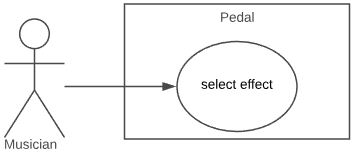
\includegraphics[width=.5\textwidth]{diagrams/use_cases/uc-select-effect.JPG}
                \caption{Select effect use case}
                \label{fig:uc-select-effect}
            \end{figure}
            
            \begin{table}[!ht]
                \centering
                \begin{tabular}{l l}
                    Use Case & Select effect \\
                    \hline \\
                    Use Case Number & 6 \\ \\
                    Summary & Musician can select an effect to use on the pedal. \\ \\
                    Actor & Musician \\ \\
                    Trigger & Hardware input: selector \\ \\
                    Pre-Conditions & The pedal must be in the modulation subsystem. \\
                    & The audio effect library must have effects. \\ \\
                    Post-Conditions & The modulation subsystem will load an effect to a cache. \\ \\
                    Assumptions & None.\\ \\
                \end{tabular}
                % \\
                % \caption{Use case: Select effect}
                % \label{tab:uc-select-effect}
            \end{table}            
            
            \paragraph{Start effect} 
            The user shall be able to start using an effect.
            \begin{figure}[!ht]
                \centering
                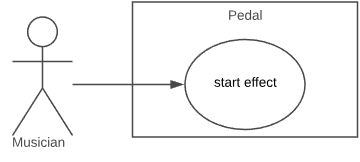
\includegraphics[width=.5\textwidth]{diagrams/use_cases/uc-effect-start.JPG}
                \caption{Start effect use case}
                \label{fig:uc-start-effect}
            \end{figure}
            \clearpage
            \begin{table}[!ht]
                \centering
                \begin{tabular}{l l}
                    Use Case & Start effect \\
                    \hline \\
                    Use Case Number & 7 \\ \\
                    Summary & Musician can start using an effect to modulate incoming audio. \\ \\
                    Actor & Musician \\ \\
                    Trigger & Hardware input: pedal toggle \\ \\
                    Pre-Conditions & The pedal must be in the modulation subsystem. \\
                    & The corresponding pedal toggle must have an effect cached. \\ \\
                    Post-Conditions & The modulation subsystem will start modulating incoming audio. \\ \\
                    Assumptions & An incoming audio signal exists.\\ \\
                \end{tabular}
                % \\
                % \caption{Use case: Start effect}
                % \label{tab:uc-start-effect}
            \end{table}     
            
            \paragraph{Stop effect} 
            The user shall be able to stop using an effect.
            \begin{figure}[!ht]
                \centering
                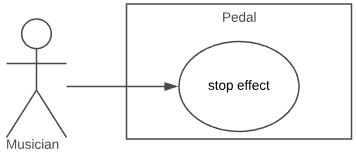
\includegraphics[width=.5\textwidth]{diagrams/use_cases/uc-effect-stop.JPG}
                \caption{Stop effect use case}
                \label{fig:uc-stop-effect}
            \end{figure}
            \begin{table}[!ht]
                \centering
                \begin{tabular}{l l}
                    Use Case & Stop effect \\
                    \hline \\
                    Use Case Number & 8 \\ \\
                    Summary & Musician can stop using an effect to modulate incoming audio. \\ \\
                    Actor & Musician \\ \\
                    Trigger & Hardware input: pedal toggle \\ \\
                    Pre-Conditions & The pedal must be in the modulation subsystem. \\
                    & An effect must be running. \\ \\
                    Post-Conditions & The modulation subsystem will stop modulating incoming audio. \\ \\
                    Assumptions & An incoming audio signal exists.\\ \\
                \end{tabular}
                % \\
                % \caption{Use case: Stop effect}
                % \label{tab:uc-stop-effect}
            \end{table}
            
\clearpage
\subsection{Composition viewpoint}

    \subsubsection{UML component diagram}
        \begin{figure}[!ht]
            \centering
            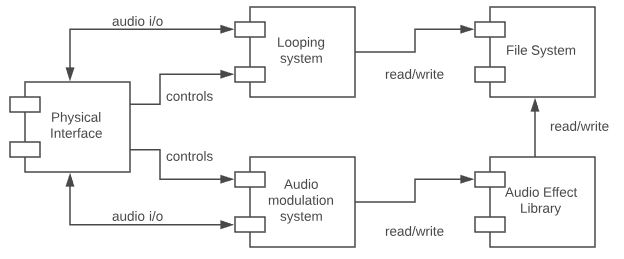
\includegraphics{diagrams/component-diagram.JPG}
            \caption{Component diagram}
            \label{fig:component}
        \end{figure}
    \subsubsection{Function attribute}
        The composition of the above entities creates the entire system to allow musicians to modulate incoming audio, or record and playback audio.
        
    \subsubsection{Subordinates attribute}
        The collection of the following entities work together to construct the working modulation/looping pedal: physical interface, looping system, audio modulation system, file system, and audio effect library.
\clearpage
\subsection{Dependency viewpoint}

    \subsubsection{UML dependency diagram}
        \begin{figure}[!ht]
            \centering
            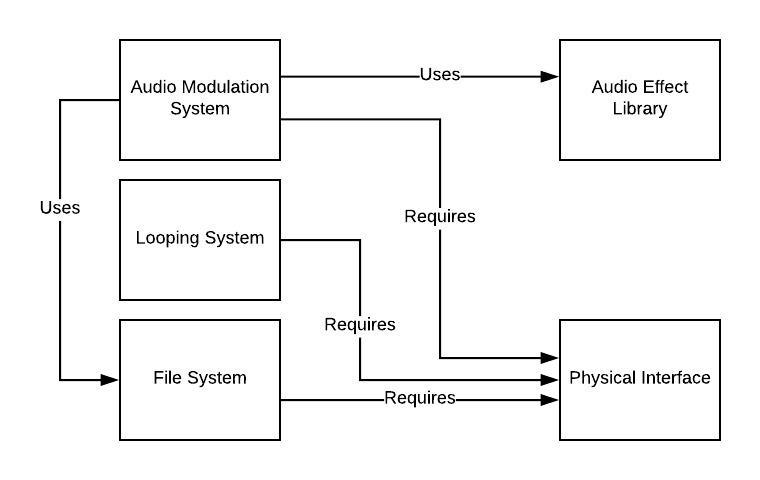
\includegraphics{diagrams/dependency-diagram.jpeg}
            \caption{Dependency diagram}
            \label{fig:dependency}
        \end{figure}
        
    \subsubsection{Dependencies attribute}
       Figure \ref{fig:dependency} shows the development dependencies for each subsystem. The first subsystems that can be designed are the Audio Modulation and Looping subsystems. The Looping subsystem design is independent from other components and can be developed at any time before the Physical Interface. The design of the Audio Modulation Subsystem is used to inform the Audio Effect Library and the File System designs. Once the software subsystems (Audio Modulation System, Looping System, and File System) are designed, work can begin on the Physical Interface design to create an interface that will adequately and efficiently control all three software subsystems.
        

\clearpage
\subsection{Interface viewpoint}
\begin{figure}[!ht]
    \centering
    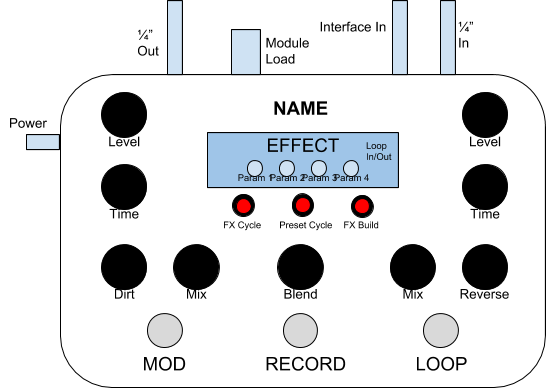
\includegraphics[width=.5\textwidth]{diagrams/pedal-diagram.png}
    \caption{Rough design diagram for the final product}
    \label{fig:pedal diagram}
\end{figure}

\subsection{Interaction viewpoint}

    \subsubsection{Looping System UML sequence diagram}
        \begin{figure}[!ht]
            \centering
            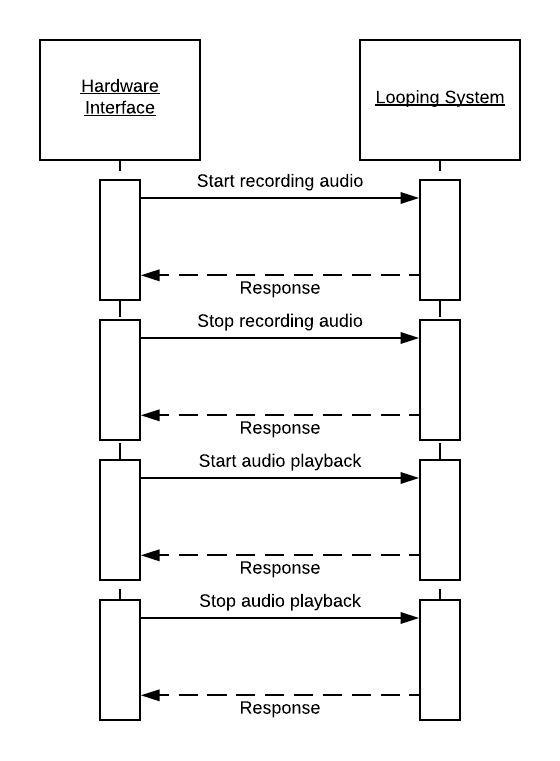
\includegraphics[width=.45\textwidth]{diagrams/looping-interaction.jpeg}
            \caption{Looping System sequence diagram}
            \label{fig:looping}
        \end{figure}
       Figure \ref{fig:looping} shows the intended interaction of the Hardware Interface and Looping Subsystem. Physical controls on the Hardware Interface correspond directly to the functionality of the Looping system. Creating a one to one relationship between the physical controls on the hardware and the software functionality they control should facilitate intuitive control while affecting the Looping System.

    \subsubsection{Audio Modulation System UML sequence diagram}
        \begin{figure}[!ht]
            \centering
            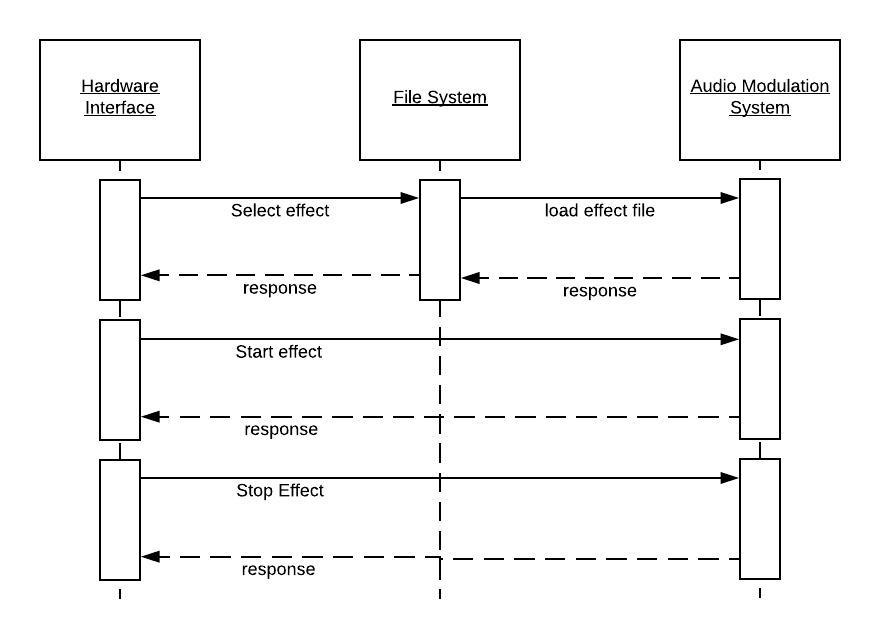
\includegraphics[width=.75\textwidth]{diagrams/modulation-interaction.jpeg}
            \caption{Audio Modulation System sequence diagram}
            \label{fig:modulation}
        \end{figure}
        Figure \ref{fig:modulation} illustrates the intended interaction between the Hardware Interface and the Audio Modulation System.
        

%\subsection{Algorithm viewpoint}
%Many of the algorithms that will need to be used already exist in the libraries we will be using. For example, csound has a built in low pass filter. 

\subsection{Resource viewpoint}
    The resources that may be present in the product, but are not part of the design are:
    \begin{itemize}
        \item External display device.
        \item Open source libraries.
        \item Any behavior related to stretch goals.
    \end{itemize}